%%%   K A L E V A L A   %%%

\documentclass{report}

\usepackage[paperwidth=130mm, paperheight=297mm]{geometry}
\usepackage[utf8]{inputenc}
\usepackage[finnish]{babel}
\usepackage{yfonts}
\usepackage{graphicx}
\usepackage[names,dvipsnames]{xcolor}
\usepackage{sectsty}

\title{\textfrak{Kalevala}}
\author{\textfrak{koonnut:\\Elias Lönnrut}}

%\usepackage{lipsum}
% Colored initial
\newcommand{\colorini}[1]{\yinipar{\textcolor{BrickRed}{#1}}}

% Define chapter title
\allsectionsfont{\color{BrickRed}\textfrak}

\begin{document}

\begin{titlepage}
    \centering
   
    \textcolor{BrickRed}{\rule{\textwidth}{1.6pt}\vspace*{-\baselineskip}\vspace*{2pt}
    \rule{\textwidth}{0.4pt}}\\[\baselineskip]
    \Huge{\textfrak{Kalevala}}
    \textcolor{BrickRed}{\rule{\textwidth}{0.4pt}\vspace*{-\baselineskip}\vspace{3.2pt}
    \rule{\textwidth}{1.6pt}}\\[\baselineskip]
    %Descriptions and Stuff \\
    %Things \\
    %Excitement\par
    \vspace*{2\baselineskip}
    
    \LARGE{\textfrak{Elias: Lönnrot}}
    
    \vfill
    {\scshape year} \\
    {\large THE PUBLISHER}\par
	\end{titlepage}
	
	\begin{figure}[ht]
		\centering
			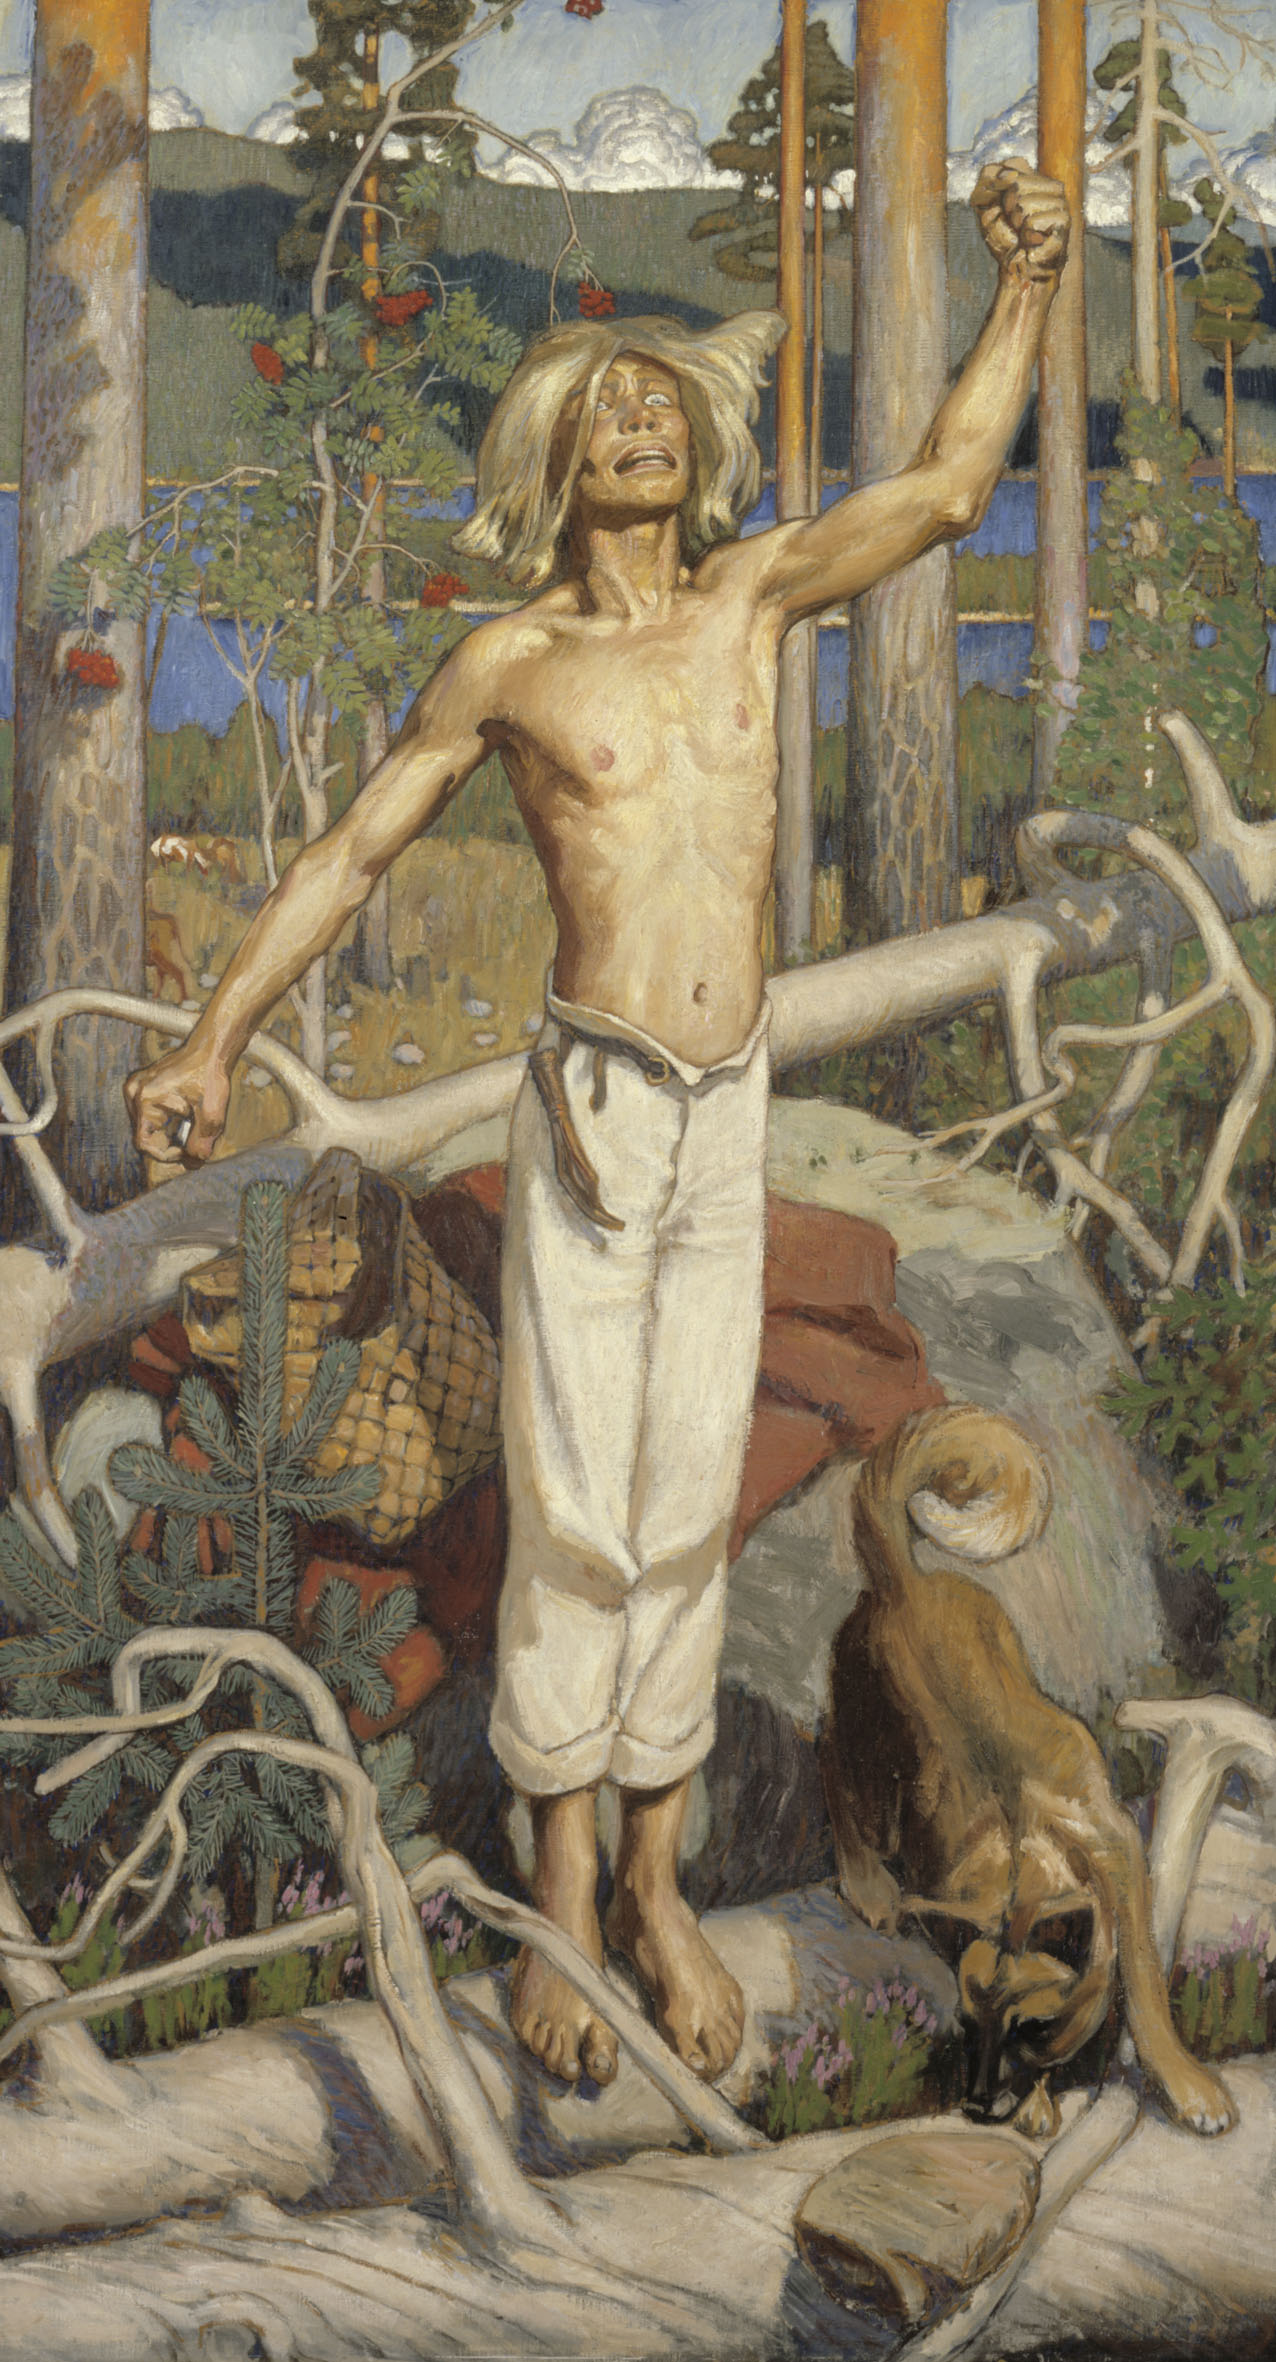
\includegraphics[width=1.00\textwidth]{./img/kullervo.png}
%		\caption{Kullervon kirous Akseli Gallen-Kallela}
%		\label{fig:kullervo}
	\end{figure}
	
	%% Ensimmäinen runo

\chapter*{Ensimmäinen Runo}

\colorini{M}{ieleni minun tekevi}, aivoni ajattelevi          \\
lähteäni laulamahan, saa'ani sanelemahan,				          	\\	
sukuvirttä suoltamahan, lajivirttä laulamahan.              \\
Sanat suussani sulavat, puhe'et putoelevat,                 \\
kielelleni kerkiävät, hampahilleni hajoovat.                \\
                                                            \\
Veli kulta, veikkoseni, kaunis kasvinkumppalini!            \\
Lähe nyt kanssa laulamahan, saa kera sanelemahan            \\
yhtehen yhyttyämme, kahta'alta käytyämme!                   \\
Harvoin yhtehen yhymme, saamme toinen toisihimme            \\
näillä raukoilla rajoilla, poloisilla Pohjan mailla.        \\
                                                            \\
Lyökämme käsi kätehen, sormet sormien lomahan,              \\
lauloaksemme hyviä, parahia pannaksemme,                    \\
kuulla noien kultaisien, tietä mielitehtoisien,             \\
nuorisossa nousevassa, kansassa kasuavassa:                 \\
noita saamia sanoja, virsiä virittämiä                      \\
vyöltä vanhan Väinämöisen, alta ahjon Ilmarisen,            \\
päästä kalvan Kaukomielen, Joukahaisen jousen tiestä,       \\
Pohjan peltojen periltä, Kalevalan kankahilta.              \\
                                                            \\
Niit' ennen isoni lauloi kirvesvartta vuollessansa;         \\
niitä äitini opetti väätessänsä värttinätä,                 \\
minun lasna lattialla eessä polven pyöriessä,               \\
maitopartana pahaisna, piimäsuuna pikkaraisna.              \\
Sampo ei puuttunut sanoja eikä Louhi luottehia:             \\
vanheni sanoihin sampo, katoi Louhi luottehisin,            \\
virsihin Vipunen kuoli, Lemminkäinen leikkilöihin.          \\
                                                            \\
Viel' on muitaki sanoja, ongelmoita oppimia:                \\
tieohesta tempomia, kanervoista katkomia,                   \\
risukoista riipomia, vesoista vetelemiä,                    \\
päästä heinän hieromia, raitiolta ratkomia,                 \\
paimenessa käyessäni, lasna karjanlaitumilla,               \\
metisillä mättähillä, kultaisilla kunnahilla,               \\
mustan Muurikin jälessä, Kimmon kirjavan keralla.           \\
                                                            \\
Vilu mulle virttä virkkoi, sae saatteli runoja.             \\
Virttä toista tuulet toivat, meren aaltoset ajoivat.        \\
Linnut liitteli sanoja, puien latvat lausehia.              \\
                                                            \\
Ne minä kerälle käärin, sovittelin sommelolle.              \\
Kerän pistin kelkkahani, sommelon rekoseheni;               \\
ve'in kelkalla kotihin, rekosella riihen luoksi;            \\
panin aitan parven päähän vaskisehen vakkasehen.            \\
                                                            \\
Viikon on virteni vilussa, kauan kaihossa sijaisnut.        \\
Veänkö vilusta virret, lapan laulut pakkasesta,             \\
tuon tupahan vakkaseni, rasian rahin nenähän,               \\
alle kuulun kurkihirren, alle kaunihin katoksen,            \\
aukaisen sanaisen arkun, virsilippahan viritän,             \\
kerittelen pään kerältä, suorin solmun sommelolta?          \\
                                                            \\
Niin laulan hyvänki virren, kaunihinki kalkuttelen          \\
ruoalta rukihiselta, oluelta ohraiselta.                    \\
Kun ei tuotane olutta, tarittane taarivettä,                \\
laulan suulta laihemmalta, vetoselta vierettelen            \\
tämän iltamme iloksi, päivän kuulun kunniaksi,              \\
vaiko huomenen huviksi, uuen aamun alkeheksi.               \\
                                                            \\
Noin kuulin saneltavaksi, tiesin virttä tehtäväksi:         \\
yksin meillä yöt tulevat, yksin päivät valkeavat;           \\
yksin syntyi Väinämöinen, ilmestyi ikirunoja                \\
kapehesta kantajasta, Ilmattaresta emosta.                  \\
                                                            \\
Olipa impi, ilman tyttö, kave luonnotar korea.              \\
Piti viikoista pyhyyttä, iän kaiken impeyttä                \\
ilman pitkillä pihoilla, tasaisilla tanterilla.             \\
                                                            \\
Ikävystyi aikojansa, ouostui elämätänsä,                    \\
aina yksin ollessansa, impenä eläessänsä                    \\
ilman pitkillä pihoilla, avaroilla autioilla.               \\
                                                            \\
Jop' on astuiksen alemma, laskeusi lainehille,              \\
meren selvälle selälle, ulapalle aukealle.                  \\
Tuli suuri tuulen puuska, iästä vihainen ilma;              \\
meren kuohuille kohotti, lainehille laikahutti.             \\
                                                            \\
Tuuli neittä tuuitteli, aalto impeä ajeli                   \\
ympäri selän sinisen, lakkipäien lainehien:                 \\
tuuli tuuli kohtuiseksi, meri paksuksi panevi.              \\
                                                            \\
Kantoi kohtua kovoa, vatsantäyttä vaikeata                  \\
vuotta seitsemän satoa, yheksän yrön ikeä;                  \\
eikä synny syntyminen, luovu luomatoin sikiö.               \\
                                                            \\
Vieri impi veen emona. Uipi iät, uipi lännet,               \\
uipi luotehet, etelät, uipi kaikki ilman rannat             \\
tuskissa tulisen synnyn, vatsanvaivoissa kovissa;           \\
eikä synny syntyminen, luovu luomatoin sikiö.               \\
                                                            \\
Itkeä hyryttelevi; sanan virkkoi, noin nimesi:              \\
"Voi poloinen, päiviäni, lapsi kurja, kulkuani!             \\
Jo olen joutunut johonki: iäkseni ilman alle,               \\
tuulen tuuiteltavaksi, aaltojen ajeltavaksi                 \\
näillä väljillä vesillä, lake'illa lainehilla!              \\
                                                            \\
"Parempi olisi ollut ilman impenä eleä,                     \\
kuin on nyt tätä nykyä vierähellä veen emona:               \\
vilu tääll' on ollakseni, vaiva värjätelläkseni,            \\
aalloissa asuakseni, veessä vierielläkseni.                 \\
                                                            \\
"Oi Ukko, ylijumala, ilman kaiken kannattaja!               \\
Tule tänne tarvittaissa, käy tänne kutsuttaessa!            \\
Päästä piika pintehestä, vaimo vatsanvääntehestä!           \\
Käy pian, välehen jou'u, välehemmin tarvitahan!"            \\
                                                            \\
Kului aikoa vähäisen, pirahteli pikkaraisen.                \\
Tuli sotka, suora lintu; lenteä lekuttelevi                 \\
etsien pesän sijoa, asuinmaata arvaellen.                   \\
                                                            \\
Lenti iät, lenti lännet, lenti luotehet, etelät.            \\
Ei löyä tiloa tuota, paikkoa pahintakana,                   \\
kuhun laatisi pesänsä, ottaisi olosijansa.                  \\
                                                            \\
Liitelevi, laatelevi; arvelee, ajattelevi:                  \\
"Teenkö tuulehen tupani, aalloillen asuinsijani?            \\
Tuuli kaatavi tupasen, aalto vie asuinsijani."              \\
                                                            \\
Niin silloin ve'en emonen, veen emonen, ilman impi,         \\
nosti polvea merestä, lapaluuta lainehesta                  \\
sotkalle pesän sijaksi, asuinmaaksi armahaksi.              \\
                                                            \\
Tuo sotka, sorea lintu, liiteleikse, laateleikse.           \\
Keksi polven veen emosen sinerväisellä selällä;             \\
luuli heinämättähäksi, tuoreheksi turpeheksi.               \\
                                                            \\
Lentelevi, liitelevi, päähän polven laskeuvi.               \\
Siihen laativi pesänsä, muni kultaiset munansa:             \\
kuusi kultaista munoa, rautamunan seitsemännen.             \\
                                                            \\
Alkoi hautoa munia, päätä polven lämmitellä.                \\
Hautoi päivän, hautoi toisen, hautoi kohta kolmannenki.     \\
                                                            \\
Jopa tuosta veen emonen, veen emonen, ilman impi,           \\
tuntevi tulistuvaksi, hipiänsä hiiltyväksi;                 \\
luuli polvensa palavan, kaikki suonensa sulavan.            \\
                                                            \\
Vavahutti polveansa, järkytti jäseniänsä:                   \\
munat vierähti vetehen, meren aaltohon ajaikse;             \\
karskahti munat muruiksi, katkieli kappaleiksi.             \\
                                                            \\
Ei munat mutahan joua, siepalehet veen sekahan.             \\
Muuttuivat murut hyviksi, kappalehet kaunoisiksi:           \\
munasen alainen puoli alaiseksi maaemäksi,                  \\
munasen yläinen puoli yläiseksi taivahaksi;                 \\
yläpuoli ruskeaista päivöseksi paistamahan,                 \\
yläpuoli valkeaista, se kuuksi kumottamahan;                \\
mi munassa kirjavaista, ne tähiksi taivahalle,              \\
mi munassa mustukaista, nepä ilman pilvilöiksi.             \\
                                                            \\
Ajat eellehen menevät, vuoet tuota tuonnemmaksi             \\
uuen päivän paistaessa, uuen kuun kumottaessa.              \\
Aina uipi veen emonen, veen emonen, ilman impi,             \\
noilla vienoilla vesillä, utuisilla lainehilla,             \\
eessänsä vesi vetelä, takanansa taivas selvä.               \\
                                                            \\
Jo vuonna yheksäntenä, kymmenentenä kesänä                  \\
nosti päätänsä merestä, kohottavi kokkoansa.                \\
Alkoi luoa luomiansa, saautella saamiansa                   \\
selvällä meren selällä, ulapalla aukealla.                  \\
                                                            \\
Kussa kättä käännähytti, siihen niemet siivoeli;            \\
kussa pohjasi jalalla, kalahauat kaivaeli;                  \\
kussa ilman kuplistihe, siihen syöverit syventi.            \\
                                                            \\
Kylin maahan kääntelihe: siihen sai sileät rannat;          \\
jaloin maahan kääntelihe: siihen loi lohiapajat;            \\
pä'in päätyi maata vasten: siihen laitteli lahelmat.        \\
                                                            \\
Ui siitä ulomma maasta, seisattelihe selälle:               \\
luopi luotoja merehen, kasvatti salakaria                   \\
laivan laskemasijaksi, merimiesten pään menoksi.            \\
                                                            \\
Jo oli saaret siivottuna, luotu luotoset merehen,           \\
ilman pielet pistettynä, maat ja manteret sanottu,          \\
kirjattu kivihin kirjat, veetty viivat kallioihin.          \\
Viel' ei synny Väinämöinen, ilmau ikirunoja.                \\
                                                            \\
Vaka vanha Väinämöinen kulki äitinsä kohussa                \\
kolmekymmentä keseä, yhen verran talviaki,                  \\
noilla vienoilla vesillä, utuisilla lainehilla.             \\
                                                            \\
Arvelee, ajattelevi, miten olla, kuin eleä                  \\
pimeässä piilossansa, asunnossa ahtahassa,                  \\
kuss' ei konsa kuuta nähnyt eikä päiveä havainnut.          \\
                                                            \\
Sanovi sanalla tuolla, lausui tuolla lausehella:            \\
"Kuu, keritä, päivyt, päästä, otava, yhä opeta              \\
miestä ouoilta ovilta, veräjiltä vierahilta,                \\
näiltä pieniltä pesiltä, asunnoilta ahtahilta!              \\
Saata maalle matkamiestä, ilmoillen inehmon lasta,          \\
kuuta taivon katsomahan, päiveä ihoamahan,                  \\
otavaista oppimahan, tähtiä tähyämähän!"                    \\
                                                            \\
Kun ei kuu kerittänynnä eikä päivyt päästänynnä,            \\
ouosteli aikojansa, tuskastui elämätänsä:                   \\
liikahutti linnan portin sormella nimettömällä,             \\
lukon luisen luikahutti vasemmalla varpahalla;              \\
tuli kynsin kynnykseltä, polvin porstuan ovelta.            \\
                                                            \\
Siitä suistui suin merehen, käsin kääntyi lainehesen;       \\
jääpi mies meren varahan, uros aaltojen sekahan.            \\
                                                            \\
Virui siellä viisi vuotta, sekä viisi jotta kuusi,          \\
vuotta seitsemän, kaheksan. Seisottui selälle viimein,      \\
niemelle nimettömälle, manterelle puuttomalle.              \\
                                                            \\
Polvin maasta ponnistihe, käsivarsin käännältihe.           \\
Nousi kuuta katsomahan, päiveä ihoamahan,                   \\
otavaista oppimahan, tähtiä tähyämähän.                     \\
                                                            \\
Se oli synty Väinämöisen, rotu rohkean runojan              \\
kapehesta kantajasta, Ilmattaresta emosta.			        		\\
	
\end{document}